\documentclass{beamer}
\usepackage[utf8]{inputenc}

\usetheme{Madrid}
\usecolortheme{default}
\usepackage{amsmath,amssymb,amsfonts,amsthm}
\usepackage{txfonts}
\usepackage{tkz-euclide}
\usepackage{listings}
\usepackage{adjustbox}
\usepackage{array}
\usepackage{tabularx}
\usepackage{gvv}
\usepackage{lmodern}
\usepackage{circuitikz}
\usepackage{tikz}
\usepackage{graphicx}
\usepackage[T1]{fontenc}
\usepackage[utf8]{inputenc}

\lstset{
  language=Python,
  basicstyle=\ttfamily\small,
  breaklines=true,
  literate={λ}{{$\lambda$}}1
}



\setbeamertemplate{page number in head/foot}[totalframenumber]

\usepackage{tcolorbox}
\tcbuselibrary{minted,breakable,xparse,skins}



\definecolor{bg}{gray}{0.95}
\DeclareTCBListing{mintedbox}{O{}m!O{}}{%
  breakable=true,
  listing engine=minted,
  listing only,
  minted language=#2,
  minted style=default,
  minted options={%
    linenos,
    gobble=0,
    breaklines=true,
    breakafter=,,
    fontsize=\small,
    numbersep=8pt,
    #1},
  boxsep=0pt,
  left skip=0pt,
  right skip=0pt,
  left=25pt,
  right=0pt,
  top=3pt,
  bottom=3pt,
  arc=5pt,
  leftrule=0pt,
  rightrule=0pt,
  bottomrule=2pt,
  toprule=2pt,
  colback=bg,
  colframe=orange!70,
  enhanced,
  overlay={%
    \begin{tcbclipinterior}
    \fill[orange!20!white] (frame.south west) rectangle ([xshift=20pt]frame.north west);
    \end{tcbclipinterior}},
  #3,
}
\lstset{
    language=C,
    basicstyle=\ttfamily\small,
    keywordstyle=\color{blue},
    stringstyle=\color{orange},
    commentstyle=\color{green!60!black},
    numbers=left,
    numberstyle=\tiny\color{gray},
    breaklines=true,
    showstringspaces=false,
}
\begin{document}

\title 
{4.6.3}
\date{September 29,2025}


\author 
{Bhoomika V - EE25BTECH11015}




\frame{\titlepage}
\begin{frame}{Question}
Find the equation of the line which passes through the point $(-2,4,-5)$ and is parallel to the line
\[
\frac{x+3}{3} = \frac{y-4}{5} = \frac{z+8}{6}.
\]
\end{frame}

\begin{frame}{The vertices of a triangle}
Let the equation of line passing through the given point be
\[
\vec{x} = 
\begin{pmatrix}
-2 \\ 4 \\ -5
\end{pmatrix}
+ \mu \vec{d}
\]
where $\vec{d}$ is the direction vector of the line.  
\end{frame}


\begin{frame}{The vertices of a triangle}
The direction vector of the line 
\[
\vec{x} = 
\begin{pmatrix}
-3 \\ 4 \\ -8
\end{pmatrix}
+ \lambda
\begin{pmatrix}
3 \\ 5 \\ 6
\end{pmatrix}
\]
is
\[
\vec{d} = 
\begin{pmatrix}
3 \\ 5 \\ 6
\end{pmatrix}.
\tag{1}
\]
\end{frame}


\begin{frame}{The vertices of a triangle}
Thus, the required equation of the line is
\[
\vec{x} =
\begin{pmatrix}
-2 \\ 4 \\ -5
\end{pmatrix}
+ \mu 
\begin{pmatrix}
3 \\ 5 \\ 6
\end{pmatrix}.
\]
\end{frame}

\begin{frame}[fragile]
    \frametitle{C Code - A function to find if triangle is right angled }

    \begin{lstlisting}
#include <stdio.h>

// Function to compute a point on the line
// Params: (px, py, pz) = point on line
//         (dx, dy, dz) = direction vector
//         t            = parameter
// Output: coords[3] = coordinates of point
void line_point(float px, float py, float pz,
                float dx, float dy, float dz,
                float t, float coords[3]) {
    coords[0] = px + dx * t;  // x = x0 + t*dx
    coords[1] = py + dy * t;  // y = y0 + t*dy
    coords[2] = pz + dz * t;  // z = z0 + t*dz
}
     \end{lstlisting}
\end{frame}

\begin{frame}[fragile]
    \frametitle{Python Code}
    \begin{lstlisting}
import numpy as np
import matplotlib.pyplot as plt
import ctypes

# --- Load the compiled C library ---
c_lib = ctypes.CDLL('./line.so')

# Define argument & return types
c_lib.line_point.argtypes = [ctypes.c_float, ctypes.c_float, ctypes.c_float,
                             ctypes.c_float, ctypes.c_float, ctypes.c_float,
                             ctypes.c_float,
                             ctypes.POINTER(ctypes.c_float)]

# --- Given point & direction vector ---
P = (-2.0, 4.0, -5.0)   # point
d = (3.0, 5.0, 6.0)     # direction vector

    \end{lstlisting}
\end{frame}

\begin{frame}[fragile]
    \frametitle{Python Code}
    \begin{lstlisting}
# --- Generate points on the line using C function ---
t_values = np.linspace(-5, 5, 50)
line_points = []

for t in t_values:
    coords = (ctypes.c_float * 3)()  # array of 3 floats
    c_lib.line_point(P[0], P[1], P[2],
                     d[0], d[1], d[2],
                     ctypes.c_float(t), coords)
    line_points.append([coords[0], coords[1], coords[2]])

line_points = np.array(line_points)

# --- Plot the line ---
fig = plt.figure(figsize=(8,6))
ax = fig.add_subplot(111, projection='3d')
    \end{lstlisting}
\end{frame}

\begin{frame}[fragile]
    \frametitle{Python Code}
    \begin{lstlisting}
ax.plot(line_points[:,0], line_points[:,1], line_points[:,2], 
        color="red", label="Required Line")
ax.scatter(P[0], P[1], P[2], color="green", s=50)
ax.text(P[0], P[1], P[2], "P(-2,4,-5)", color="green")

# Labels
ax.set_xlabel("X-axis")
ax.set_ylabel("Y-axis")
ax.set_zlabel("Z-axis")
ax.set_title("Line through P(-2,4,-5) with direction (3,5,6)")
ax.legend()
plt.show()
    \end{lstlisting}
\end{frame}

\begin{frame}{Plot}
    \centering
    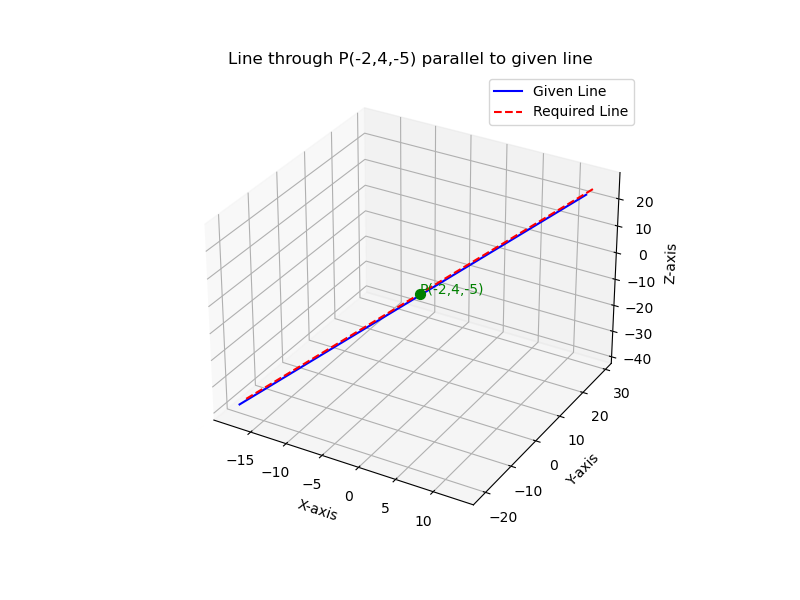
\includegraphics[width=\columnwidth, height=0.8\textheight, keepaspectratio]{Figs/Fig1.png}     
\end{frame}

\end{document}